%%%%%%%%% PROJECT DESCRIPTION  -- 15 pages (including Prior NSF Support)

\required{Project Description}
\begin{center}
%\emph{Maximum of 15 pages}
\end{center}
%The Project Description (including Results from Prior NSF Support, which is
%limited to five pages) may not exceed 15 pages. Visual materials, including charts,
%graphs, maps, photographs and other pictorial presentations are included in the
%15-page limitation. PIs be cautioned that the project description must
%be self-contained and that URLs that provide information related to the proposal
%should not be used. \\
%
%All proposals to NSF are reviewed utilizing the two merit review criteria,
%intellectual merit and broader impacts. \\
%
% The Project Description should provide a clear statement of the work 
% to be undertaken and must include: objectives for the period of the proposed 
% work and expected significance; relation to longer-term goals of the PI's 
% project; and relation to the present state of knowledge in the field, 
% to work in progress by the PI under other support and to work in progress 
% elsewhere.

%%%%%%%%%%%%%%%%%%%%%%%%%%%%%%%%%%%%%%%%%%%%%%%%%%%%%%%%%%%%%%%%%%%%%%
%INTRO
%%%%%%%%%%%%%%%%%%%%%%%%%%%%%%%%%%%%%%%%%%%%%%%%%%%%%%%%%%%%%%%%%%%%%%
\section*{Introduction}

While the potential role of hybridization and introgression as agents of evolution has long been appreciated \citep{Anderson1948, Anderson1954, Stebbins1959}, only recently have technological innovations allowed for characterization of these processes on a genome-wide scale. 
Multiple studies have now reported substantial inter-taxon introgression in both plant \citep{Hufford2013, renaut2013} and animal \citep{consortiumbutterfly2012, staubach2012, huerta2014} species, and introgression has been found across considerable portions of genomes and specifically at loci thought to underlie adaptation. 

In the investigation proposed here, we will build upon our previous work in maize (\emph{Zea mays} ssp. \emph{mays}) and its wild relatives the teosintes (\emph{Zea} spp.) to characterize the evolutionary role of hybridization and introgression in this system and more generally describe how these processes can shape genomes. 
As a study system, the genus \emph{Zea} is ideally suited for such research due to the distribution of large, natural populations across a range of environments and the availability of exceptional genomic resources \citep{Hufford2012}.  Within \emph{Zea} we will be able to assess the genome-wide effects of hybridization and introgression at two different timescales.  
First, analysis of hybridization and divergence between the subspecies \emph{Zea mays} ssp. \emph{parviglumis} and \emph{Zea mays} ssp. \emph{mexicana} will generate basic knowledge of the process of incipient speciation and the porous nature of genomes of diverging species on an evolutionary timescale ($\sim60,000$ generations).
Second, evaluation of introgression in sympatric maize and teosinte on the ecological timescale ($\sim3,000-9,000$ generations) during which domesticated maize colonized the Americas will inform our understanding of the role of introgression in adaptation to new or rapidly changing environments.   

%%%%%%%%%%%%%%%%%%%%%%%%%%%%%%%%%%%%%%%%%%%%%%%%%%%%%%%%%%%%%%%%%%%%%%
%OBJECTIVES
%%%%%%%%%%%%%%%%%%%%%%%%%%%%%%%%%%%%%%%%%%%%%%%%%%%%%%%%%%%%%%%%%%%%%%
\section*{Objectives}
	
%We will leverage the resources of the \emph{Zea} study system to address two primary objectives:

\subsection*{Objective I: Assess the evolutionary and genomic effects of hybridization in locally-adapted, parapatric wild teosinte}
\emph{Zea mays} ssp. \emph{parviglumis} (the wild progenitor of maize; hereafter, \emph{parviglumis}) and \emph{Zea mays} ssp. \emph{mexicana} (hereafter, \emph{mexicana}) diverged approximately 60,000 BP \citep{Ross-Ibarra2009a} and have parapatric distributions: while \emph{parviglumis} occurs in the warm lowlands of southwest Mexico, \emph{mexicana} is found in the cool highlands of the Central Plateau. Narrow regions of admixture between these wild subspecies have been discovered at middle elevations \citep{Fukunaga2005, Pyhajarvi2013}. 
Through targeted collections, generation of high-density genotyping data, population genomic analyses, and common garden experiments, we will address the following research questions:
\begin{enumerate}
\item \emph{What fraction of the genome is porous to gene flow in hybrid zones?}

\item \emph{How do the fitness of parental and hybrid populations vary across the hybrid zone?}

\item \emph{Is there evidence of selection on putatively adaptive traits across hybrid zones?}
\end{enumerate}
\vspace{0.5cm}

\subsection*{Objective II: Determine the extent to which hybridization and introgression have altered the \emph{Zea} genus during the post domestication spread of maize}
Maize was domesticated in southwest Mexico from \emph{parviglumis} $\sim$9,000 BP \citep{Matsuoka2002} and quickly spread throughout the Americas, bringing this crop into sympatry with new species of teosinte \citep{Vigouroux2008a}. Through a combination of dense genotyping of range-wide samples of maize and teosinte and targeted, full-genome sequencing we will assess three questions regarding the importance of introgression during the spread of maize:
\begin{enumerate}
\item \emph{Was the spread of maize facilitated by gene flow from locally-adapted wild \emph{Zea}?}
\item \emph{What is the geographic scale of adaptive introgression?}
\item \emph{Did maize serve as a bridge for gene flow between isolated \emph{Zea} taxa?}
\end{enumerate}

%%%%%%%%%%%%%%%%%%%%%%%%%%%%%%%%%%%%%%%%%%%%%%%%%%%%%%%%%%%%%%%%%%%%%%
%RATIONALE AND SIGNIFICANCE
%%%%%%%%%%%%%%%%%%%%%%%%%%%%%%%%%%%%%%%%%%%%%%%%%%%%%%%%%%%%%%%%%%%%%%
\section*{Rationale and Significance}
Pioneers in evolutionary biology including G. Ledyard Stebbins and Edgar Anderson recognized the important role hybridization and introgression could play in adaptation and speciation \citep{Anderson1948, Anderson1954}. These evolutionary forces were thought to be particularly influential when environmental conditions encountered by a species were marginal, variable, or new \citep{Stebbins1959}. More recently, defined and stable regions of hybridization, referred to as hybrid zones, have been discovered in a number of taxa \citep[reviewed in ][]{HarrisonHybridZone, shurtliff2013, abbott2014}. Increasingly, it is clear that the phenomena of hybridization and subsequent introgression shape genomes and influence the trajectory of species as they evolve. Hybridization has long been believed to play a role in speciation, and introgression of even a small number of loci can enable a species to adapt and invade novel habitats \citep{currat2008, abbott2013}.  For example, we now have strong molecular evidence that hybridization has led to speciation in both plants and animals \citep[reviewed in][]{mallet2007}, that non-native species have been facilitated in invasions through hybridization \citep[\emph{e.g.}, the expansion of sticklebacks in Switzerland:][]{lucek2010}, and that crops were aided by introgression from locally-adapted wild relatives during their global spread from narrow centers of origin \citep{he2011, Hufford2013}.

While theory regarding hybridization has progressed and many compelling empirical examples have been identified, several outstanding questions remain. 
Additional common garden studies are needed to determine whether hybrid zones are primarily maintained as tension zones in which hybrids are selected against or as ecotones where hybrids have an advantage under certain environmental conditions \citep{Kruuk1999, Rasmussen2012, Smith2013b}. 
Moreover, genome-wide analysis of the fraction of the genome that is porous to gene flow in hybrid zones is rare and will likely offer considerable insight.  
For example, recent genomic studies of introgression suggest that rates of gene flow vary substantially across loci, likely as a function of selection for or against introgressed alleles \citep{Hufford2013, Poelstra2014}.  
In addition, chromosomal rearrangements (\emph{e.g.}, inversions and translocations) likely play an important role in adaptation and structuring introgression along the genome and may restrict gene flow in hybridizing species \citep{guerrero2012, Barb2014, guerrero2014}.

 	 
Both wild and domesticated \emph{Zea} offer exciting opportunities to study hybridization. 
The subspecies \emph{parviglumis} and \emph{mexicana} are distributed across a steep altitudinal gradient and differ for traits that are thought to be adaptive in the highlands such as the presence of macrohairs, stem pigmentation and shorter flowering time in \emph{mexicana}.
A recent ecological niche study has found that distributions of these subspecies are quite unique and stable over many thousands of years \citep{hufford2012inferences}.
However, analysis of microsatellite markers genotyped in a range-wide sample has identified elevated admixture between the subspecies in two geographically-distinct, mid-elevation regions of Mexico between the distributions of both parental species, suggesting the presence of multiple hybrid zones \citep{Fukunaga2005}.  
Our recent genome-wide analysis of a population in one of these hybrid zones revealed extensive subspecies admixture across all individuals sampled and relatively short shared haplotypes with individuals from populations of non-admixed \emph{parviglumis} or \emph{mexicana} \citep{Pyhajarvi2013}.
This suggests continual gene flow between \emph{parviglumis} and \emph{mexicana} in this hybrid zone over a substantial period of time \citep{Pyhajarvi2013}.  
Longer shared haplotypes were found in the hybrid population in chromosomal regions identified as potential inversions \citep{Pyhajarvi2013}.  
These regions may be particularly resistant to gene flow between subspecies, but may also prove adaptive for individuals in some parts of the hybrid zone.
Very little is known, however, about the patterns of hybridization in other populations in this region or in other hybrid zones.
Hybrid populations of \emph{mexicana} and \emph{parviglumis} are distributed across elevation gradients in markedly different regions of Mexico and are found at varying distances from each subspecies.
By expanding our preliminary studies we can assess whether similar dynamics occur in replicate populations and zones and determine if specific loci are consistently introgressed and widely adaptive or, rather, tied to specific habitats.

In addition to the ongoing hybridization between \emph{parviglumis} and \emph{mexicana} that has likely occurred since their divergence $\sim$60,000 BP, gene flow between domesticated maize and various taxa of the genus \emph{Zea} has been detected based on both hybrid morphologies observed in the field \citep{wilkes1967teosinte, Wilkes1977} and genetic data \citep{Fukunaga2005,Ross-Ibarra2009a}. 
Maize domestication from \emph{parviglumis} occurred recently on an evolutionary timescale \citep[$\sim$9,000BP][]{Matsuoka2002}) and was followed by rapid spread of the crop across the Americas over the following millennia \citep{Piperno2001,Grobman2012}. 
During this diffusion, maize was brought into sympatry with new wild relatives that were likely allopatric to the progenitor of maize (\emph{i.e., parviglumis}) for long periods prior to domestication \citep{hufford2012inferences}. 
Our recent work has provided evidence of introgression from \emph{mexicana} into maize during its earliest expansion into the highlands of the Mexican Central Plateau.  
We found consistent introgression into several highland maize populations at QTL for phenotypes (\emph{e.g.}, pigment and macrohairs) that distinguish highland \emph{mexicana} from lowland \emph{parviglumis} teosinte, and showed that \zm{} phenotypes and higher growth rate were found in maize plants with \emph{mexicana} introgression \citep{Hufford2013}.
Our interpretation of these results is that maize received adaptive introgression from \emph{mexicana} that allowed the crop to spread into the highlands of Mexico. 

Subsequent to its diffusion into the Mexican highlands, maize spread into sympatry with additional teosinte taxa in Guatemala including \emph{Zea luxurians} (hereafter, \emph{luxurians}) and \emph{Zea mays} ssp. \emph{huehuetenangensis} (hereafter, \emph{huehuetenangensis}), each adapted to environmental conditions very different from those of the progenitor \emph{parviglumis}. 
Although maize is known to hybridize with both taxa, the extent and adaptive significance of gene flow between these teosintes and maize is unknown.  
Based on analysis of a small number of resequenced loci, \emph{mexicana} haplotypes appear to be segregating in \emph{luxurians} \citep{Ross-Ibarra2009a}.  
Since \emph{mexicana} and \emph{luxurians} are entirely allopatric in their distributions, this suggests maize may have served as a bridge for gene flow between these two taxa.  
Further work will be necessary to explore this possibility and to assess if maize has, more generally, altered the genomes of \emph{Zea} species through gene flow during its spread across the Americas (see \ref{ss:genuswide}).

Through the targeted studies we propose here in the genus \emph{Zea}, we will address basic evolutionary questions that are relevant across systems including:
\begin{itemize}\itemsep0pt
\item Do chromosomal regions that are resistant to introgression or commonly introgressed in a hybrid zone associate with fitness or putatively adaptive phenotypes?
\item How do hybrid zone dynamics depend on environment and are they replicable across zones?
\item Does gene flow from native relatives allow a colonizing/invasive species to more readily adapt to new environments?
\item At what geographical scale do introgression and local adaptation interact?
\item Can a widespread congener act as a bridge for gene flow between smaller allopatric taxa?
\end{itemize}

%%%%%%%%%%%%%%%%%%%%%%%%%%%%%%%%%%%%%%%%%%%%%%%%%%%%%%%%%%%%%%%%%%%%%%
%PRELIMINARY RESULTS
%%%%%%%%%%%%%%%%%%%%%%%%%%%%%%%%%%%%%%%%%%%%%%%%%%%%%%%%%%%%%%%%%%%%%%
\section*{Preliminary Results}

Our previous publications suggest \emph{Zea} is a promising model system for exploring the evolutionary role of hybridization and introgression (\emph{e.g.},  \citealt{Ross-Ibarra2009a, vanheerwaarden2011a, Hufford2013, Pyhajarvi2013}).  To further refine our research questions and provide preliminary results for this proposal we have reanalyzed published data  \citep{Fang2012} of 983 SNPs genotyped across a panel of $>2,000$ samples including all subspecies and species of teosinte and an Americas-wide sample of maize landraces (\emph{i.e.}, traditional open-pollinated varieties).  While the low density of markers in these data precludes genome-wide inferences and haplotype-based analyses, the comprehensive taxon sampling makes this an ideal resource for guiding future research.

\subsection*{Evidence for hybrid zones between \emph{parviglumis} and \emph{mexicana}}

Using the \citet{Fang2012} data, we calculated the probability of each sample's assignment to \emph{parviglumis} and \emph{mexicana} groups using STRUCTURE \citep{Pritchard2000}.  We find that individuals from several mid-elevation populations show appreciable assignment to both \emph{parviglumis} and \emph{mexicana} groups (Figure \ref{fig:structure}) and likely represent hybrid populations.  

\begin{figure}[h!] 
  \centering
   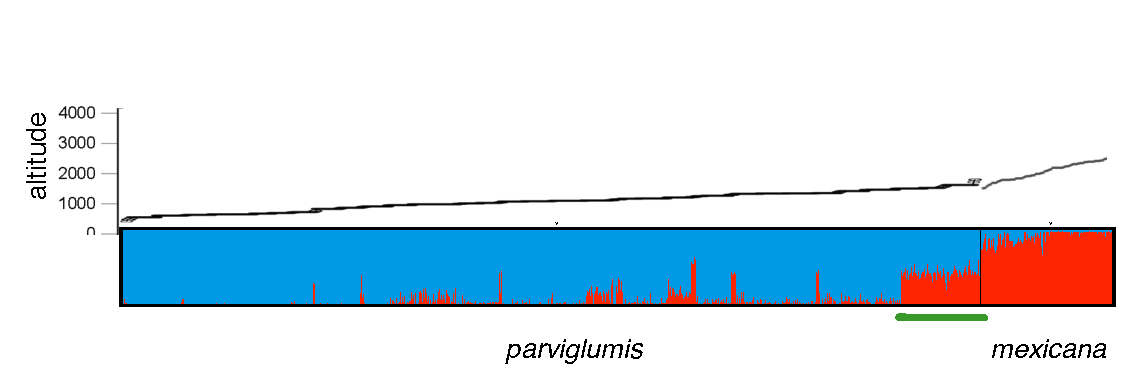
\includegraphics[width=0.95\textwidth]{structure.pdf}
    \caption{Assignment of \emph{parviglumis} and \emph{mexicana} individuals to K=2 groups using the Bayesian assignment algorithm of STRUCTURE \citep{Pritchard2000}.  Individuals are sorted by increasing altitude as indicated by the plot above the bar chart. Individuals from mid-elevation, hybrid zone populations are underscored in green.} 
\label{fig:structure}
\end{figure}

Admixed populations cluster in two geographically distinct regions of Mexico: the eastern Balsas River Basin and eastern Jalisco state.  These locations fall at intermediate locations between the main distributions of \emph{parviglumis} and \emph{mexicana} (Panel A, Figure \ref{fig:pies}).  Hybrid populations from eastern Jalisco state are found at higher elevation (mean 1632m) than those in the eastern Balsas (mean 1531m) and also show a higher proportion of membership in the highland teosinte \emph{mexicana} (Panels B and C, Figure \ref{fig:pies}).  These findings suggest that hybrid populations from distinct environments may vary in the proportion of ancestry from each subspecies in a manner that is adaptive. Estimates of pairwise population differentiation also suggest that hybrid populations in the Balsas and Jalisco are distinct in that Jalisco populations are less differentiated from \emph{mexicana} than hybrid populations in the Balsas (Table \ref{tab:Fst}).  Not surprisingly, populations in both hybrid zones are less differentiated from \emph{mexicana} and \emph{parviglumis} than these subspecies are from each other. 

\begin{figure}[h!]
  \centering
   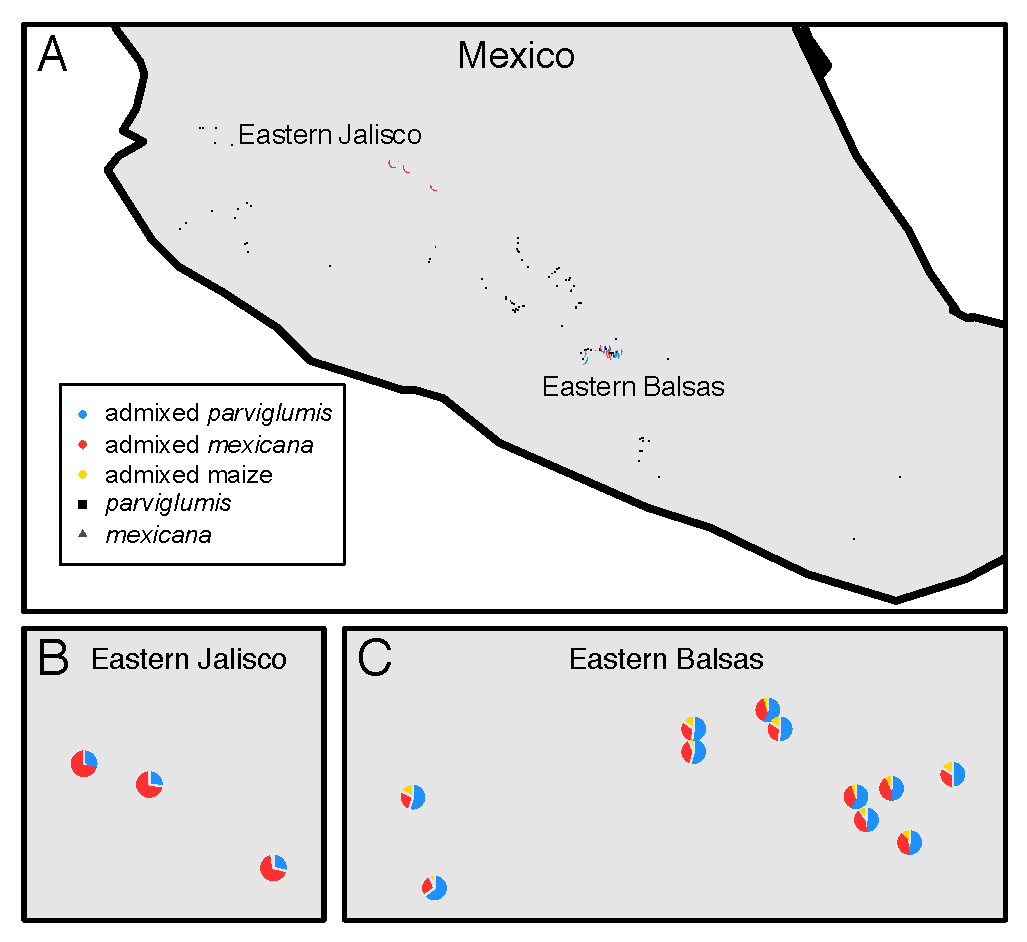
\includegraphics[width=0.6\textwidth]{map.pdf}
    \caption{A) Location of two putative hybrid zones of \emph{mexicana} and \emph{parviglumis}.  Hybrid populations are represented as pie charts with proportion assigned to \emph{mexicana}, \emph{parviglumis}, and maize groups. Zoomed-in views of the Eastern Jalisco (B) and Eastern Balsas (C) hybrid populations.} 
\label{fig:pies}
\end{figure}

\begin{table}[h!]
\rowcolors{2}{gray!25}{white}
\begin{center}
\caption{Pairwise $F_{ST}$ between teosinte and hybrid populations} \label{tab:Fst}
\begin{tabular}{lcccc}\\\toprule
{\bf Taxon}&{\bf \emph{parviglumis}}&{\bf \emph{mexicana}}&{\bf Jalisco Hybrids}&{\bf Balsas Hybrids}\\\midrule
{\bf \emph{parviglumis}}&---&---&---&---\\
{\bf \emph{mexicana}}&0.107&---&---&---\\
{\bf Jalisco Hybrids}&0.059&0.064&---&---\\
{\bf Balsas Hybrids}&0.057&0.074&0.034&---\\\bottomrule
\end{tabular}
\end{center}
\end{table} 

\subsection*{Evidence for introgression across \emph{Zea}}

Our initial survey of divergence and gene flow in \emph{Zea}, based on a set of 26 Sanger-sequenced loci, found evidence for admixture between allopatric populations of \emph{mexicana} and \emph{luxurians} at multiple loci \citep{Ross-Ibarra2009a}. 
As there is no evidence to suggest that these populations overlapped in their recent history, we took these results to suggest that maize, which is known to hybridize with both taxa, may have served as a bridge for gene flow between them.
Further support for this idea comes from patterns of haplotype segregation at an inversion locus on chromosome 4 \citep[\emph{Inv4m};][]{Fang2012,Pyhajarvi2013,Hufford2013}. 
The inverted haplotype at this locus appears to be derived in \emph{mexicana} \citep{Pyhajarvi2013}.
This haplotype has introgressed from \emph{mexicana} into maize in the highlands of Mexico, an apparent example of adaptive introgression \citep[Panel A, Figure \ref{fig:hufmap};][]{Hufford2013}.
A SNP allele from the 983-SNP set is diagnostic for the inverted \emph{mexicana} haplotype.
We have screened the $>2000$ samples in this data set for this allele and have found that the \emph{mexicana} haplotype is segregating in maize in the highlands of both Mexico and Guatemala (Panel B, Figure \ref{fig:hufmap}).  The haplotype is also present in all samples of \emph{luxurians} genotyped in \citet{Fang2012}.
These preliminary results suggest that the inversion has moved from \emph{mexicana} into \emph{luxurians} via a maize intermediate.

\begin{figure}[h!]
  \centering
   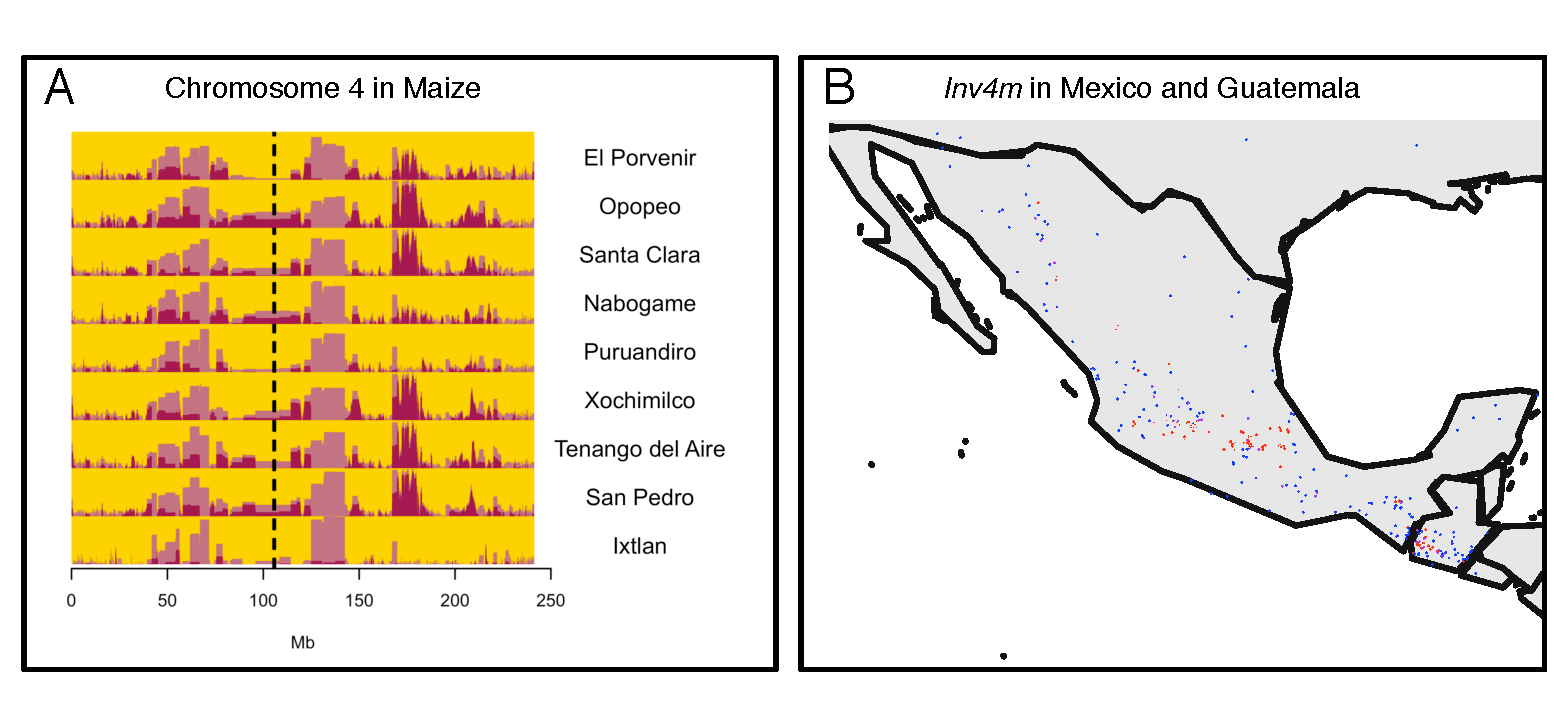
\includegraphics[width=1\textwidth]{inv_map.pdf}
    \caption{A) Introgression from \zm\ to maize along chromosome 4.  Each row represents a population of maize, and the proportion of individuals with a \zm\ allele at a given position along the genome is shown in dark red.  Light red represents chromosomal regions identified as having a high false positive rate in null permutations.  The strong signal of introgression at Mb 180 is the inversion polymorphism \emph{Inv4m}. B) Geographic distribution of alleles at a SNP found to be diagnostic of the \emph{Inv4m} inversion.  Genotypes are shown in color (blue: homozygous standard, purple: heterozygous, red: homozygous inverted) and shapes represent taxa (squares: \zm, triangles: \zp, circles: domesticated maize)} 
\label{fig:hufmap}
\end{figure}
%%%%%%%%%%%%%%%%%%%%%%%%%%%%%%%%%%%%%%%%%%%%%%%%%%%%%%%%%%%%%%%%%%%%%%
%SPECIFIC OBJECTIVES
%%%%%%%%%%%%%%%%%%%%%%%%%%%%%%%%%%%%%%%%%%%%%%%%%%%%%%%%%%%%%%%%%%%%%%
\section*{Research Plan}

\subsection{Evolutionary genomics of a teosinte hybrid zone}
\label{ss:hybrids}
\subsubsection{What fraction of the genome is porous to gene flow in hybrid zones?}
\label{sss:genomescan}
Recent studies have suggested the functional architecture of genomes can lead to chromosomal regions of high differentiation in hybridizing species \citep{renaut2013}, but these regions are not always conserved across populations \citep{Parchman2013}. Currently, few studies have dissected the genome-wide architecture of hybridization in replicate hybrid zones, and little is known about the consistency of genome porosity to gene flow. Genome-wide studies in teosinte are feasible at high marker density \citep{Hufford2012b, Hufford2013, Pyhajarvi2013} and are informed by the genomic resources of maize \citep{Hufford2012}, often providing functional annotation for loci of interest, a rarity in other natural systems.  The Hufford Laboratory and Senior Personnel Luis Eguiarte will assess the genomic architecture of hybridization evidence for selection in two hybrid zones of \emph{mexicana} and \emph{parviglumis} through population collections, generation of genotype and sequence data, and application of population genomic analyses appropriate to this question. 

\paragraph{\emph{Panel Construction and Sample Collection:}}
From previous collections, we have access to an extensive sampling of \emph{parviglumis}, \emph{mexicana}, and maize from throughout their respective ranges.  Moreover, Senior Personnel Luis Eguiarte and collaborator Salvador Montes-Hernandez (see attached letter of commitment) have recently collected altitudinal transects of \emph{parviglumis} and \emph{mexicana} that extend through both hybrid zones targeted by our project \citep{Diez2013} and are  familiar with populations in this region.  Our current collections will likely be insufficient for both the genotyping and common garden activities we propose  and we have therefore budgeted for a collection trip during the first year of the project.  We will collect from 15 sampling sites in each of 16 populations.  Sampling sites will be randomly stratified across the elevation gradient of each population.  At each sampling site we will collect as much seed as possible from each of five teosinte plants.  In the wild, teosinte plants produce, on average, 100 seeds per plant \citep{wilkes1967teosinte}.  We will also measure plant density, slope of the terrain, and canopy cover at each sampling site.  These data will be useful covariates for estimating any potential maternal effects in our common garden experiments.  Four populations will be sampled from both the eastern Jalisco and eastern Balsas hybrid zones.  To the extent possible, we will select hybrid populations in a stratified manner across the elevation gradient found in these regions. Four populations each will also be collected from non-admixed \emph{parviglumis} and \emph{mexicana}, with two populations of each taxon collected from regions proximate to both hybrid zones.  We have already obtained the requisite collection permits as well as permits for importing samples into the United States for genetic analysis. Following collection, samples will be sent to the lab of Dr. Eguiarte at the Universidad Nacional Aut\'{o}noma de M\'{e}xico (UNAM) for cold storage until common garden experiments are planted (see \ref{sss:fitness}).  During year two of our proposed project, leaf tissue will be collected from a single plant per sampling site ($n=240$) in our mid-elevation common garden (see \ref{sss:fitness}) at the 5-7 leaf stage, stored in silica, and shipped to Iowa State University for DNA isolations and subsequent genotyping and full-genome sequencing.

\paragraph{\emph{Sample Genotyping and Sequencing:}}
DNA for genotyping will be isolated using a modified CTAB procedure \citep{Saghai-Maroof1984}.  For sample genotyping ($n=240$) we will utilize the services of the Genomic Diversity Facility at Cornell University to implement a reduced representation approach to next-generation sequencing called Genotyping By Sequencing (GBS; \citealt{Elshire2011}; see attached letter of commitment from Sharon Mitchell). To date, this method has been implemented to genotype tens of thousands of maize samples and a bioinformatics pipeline (TASSLE-GBS) has been constructed that allows for genotyping $\sim$1,000,000 SNPs in maize \citep{Glaubitz2014} using standard GBS data. 
We will multiplex only 48 individuals per lane (instead of the standard 384 used for inbred lines) to minimize missing data and errors in identifying heterozygote genotypes.
We have already successfully applied GBS to heterozygous maize and teosinte and find that, even after filtering for missing data, GBS provides many more markers with minimal ascertainment bias at a fraction of the cost of other available technologies. 

In addition to GBS data, we will generate full-genome sequence through the Iowa State University DNA Facility for a single hybrid individual from each hybrid zone.  We will generate two lanes of Illumina HiSeq 150bp, paired-end data per individual.  
We have previous experience dealing with whole genome shotgun data \citep{Gore2009,Chia2012a,Hufford2012b}, and have recently developed and implemented an open-source pipeline for read-mapping and SNP calling (\url{https://github.com/RILAB/paap}) using the existing maize B73 reference genome.

\paragraph{\emph{Population Genomic Analyses:}} 
We will assess the genome-wide patterns of ancestry using several approaches.  
First, standard measures of differentiation including $F_{ST}$, the proportion of shared and fixed variants, and relative levels of nucleotide diversity \citep{Geneva2014} will be calculated in sliding windows along the genome. 
Second, we will attempt to implement haplotype-based methods for detecting introgression \citep[\emph{e.g.},][]{price2009, lawson2012} that will effectively allow us to model chromosomes from hybrid populations as mosaics of reference allopatric populations of \emph{parviglumis} and \emph{mexicana}.  
Finally, if phasing genotypes \citep{scheet2006fast} proves difficult given high levels of missing data or heterozygous error, we will make use of software designed to estimate admixture from genotype-likelihoods calculated on low-coverage sequence data \citep{skotte2013estimating}. 
We have already designed pipelines to work with genotype-likelihoods (e.g. \url{https://github.com/rossibarra/angsbigd}) and can utilize these methods to calculate standard diversity statistics.  
We will assess excess of \emph{parviglumis} or \emph{mexicana} ancestry on a site-by-site basis across hybrid genomes at the population level and will determine whether patterns are conserved across populations within hybrid zones and between hybrid zones.  Chromosomal regions showing an excess of ancestry from one taxon in hybrid populations will be inspected for evidence of selection using a combination of site-frequency-, linkage-disequilibrium-, and population-differentiation-based methods \citep[reviewed in][]{Vitti2013}. Chromosomal regions showing strong evidence of selection across individuals within a hybrid zone based on analysis of GBS data will be further dissected using high-density, full-genome data generated for a single individual per hybrid zone.  
Whole genome sequence will allow definition of the exact haplotype(s) that have introgressed, allowing estimation of the age of the introgression and potentially identifying candidate causal polymorphisms.  

\subsubsection{How do the fitness of parental and hybrid populations vary across the hybrid zone?} 
\label{sss:fitness}
In order to assess fitness and variation at putatively adaptive traits across both non-admixed and  hybrid populations we will conduct common garden experiments in Mexico at three altitudes: 1) Below a hybrid zone in habitat occupied by non-admixed \emph{parviglumis}; 2) Within hybrid zone habitat; and 3) Above a hybrid zone in habitat occupied by non-admixed \emph{mexicana}. 
Common garden experiments will be replicated over years two and three of our proposed project.  

Discussions with collaborators in Mexico (Ruairidh Sawers and Salvador Montes-Hernandez; see attached letters of commitment) raised concerns about the safety of students at field sites in the state of Guerrero (the location of the eastern Balsas hybrid zone; see US State Department Travel Warning at \url{http://travel.state.gov/content/passports/english/alertswarnings/mexico-travel-warning.html}) and the feasibility of managing six concurrent gardens. We thus propose a single transect of three replicate gardens in the eastern Jalisco hybrid zone. 
In our initial discussions with Drs. Sawers and Montes-Hernandez we have identified potential high- and low-elevation sites near Celaya and Bucerias, Mexico respectively.  
We will explore options for our third hybrid zone garden during our collections in the first year of the project.
The hybrid zone is less than 50 kilometers from the host institution of Dr. Sawers (Langebio in Irapuato, Mexico) and identification of an appropriate site should be straight-forward.
Each garden will consist of three complete blocks including a randomization of three plants from each of 15 sampling sites in the 16 populations described in \ref{sss:genomescan} (3 blocks x 3 plants x 15 sites x 16 populations = 2,160 plants per garden).  We will measure fitness-related phenotypes (percent germination, germination rate, plant height at 15-day intervals, seed set, 50-seed weight, total-above-ground biomass, stomatal conductance and survival), putatively adaptive traits across the altitudinal gradient (macrohair density, pigmentation extent, and flowering time) and traits for which there is no \emph{a priori} evidence of selection across an elevational gradient (culm diameter and the width of the leaf beneath the first lateral branch at the time of flowering).  Analysis of relative fitness of hybrid, \emph{parviglumis} and \emph{mexicana} plants across our garden sites will allow provide evidence regarding ecotone vs. tension zone dynamics in teosinte hybrid zones.  Ecotone dynamics would be supported by hybrids possessing the highest fitness of all plants in the mid-elevation gardens, whereas tension zone dynamics would be supported by hybrids having lower fitness in all gardens.  Phenotypic data for putatively adaptive traits and traits with no evidence of selection will be analyzed in \ref{sss:driftsel}.
		
\subsubsection{Is there evidence for selection on putatively adaptive traits across hybrid zones?}
\label{sss:driftsel}
Stem pigmentation, macrohair density, and flowering time in particular are thought to be under selection in teosinte across an elevational gradient.  Pigmented and pilose plants have an advantage in retaining heat at high elevation (for a discussion of highland adaptation in the context of maize see \citealt{Eagles1994}). Additionally, \emph{mexicana} flowers much earlier than \emph{parviglumis} \citep{Rodriguez2006}, which may represent an adaptation to shorter growing seasons at high elevation. We will combine our genome-wide marker data obtained in \ref{sss:genomescan} with phenotypic data collected in our common garden experiments in \ref{sss:fitness} in order to evaluate evidence for selection on these potentially adaptive traits.  A method recently developed by \citet{Ovaskainen2011} and implemented in the software DRIFTSEL \citep{Karhunen2013} is particularly suited to this purpose.  The method builds upon the $F_{ST}$--$Q_{ST}$ framework for comparison of population differentiation and quantitative trait divergence and allows the signature of selection on a given phenotypic trait to be distinguished from genetic drift.  The strength of evidence for selection based on DRIFTSEL for putatively adaptive traits (pigment, macrohairs, flowering time) will be compared to that of traits with no \emph{a priori} evidence of selection across an elevational gradient (culm diameter and leaf width).

In addition, we will conduct association analyses to connect genotype to phenotype using GBS data described in \ref{sss:genomescan} and phenotypic data for potentially adaptive traits and traits gauging fitness.  Association analysis will be conducted using TASSEL5.0 \citep{Bradbury2007}. Significant associations will then be cross-referenced with regions of excess ancestry from \emph{parviglumis} or \emph{mexicana} in hybrid populations and zones identified in \ref{sss:genomescan}, particularly those that show evidence of selection based on additional population genetic summary statistics.  This final combination of data and analyses could reveal the traits, loci, and ancestry source under selection within hybrid zones.

\subsection{Crop-wild introgression during maize diffusion} \label{ss:genuswide}

%\jri{i like having an intro that ties together the questions. i think some of the text from rational could go here and in your objective 1 above. i still think the rational/significance should address not what the questions are in teosinte per se, but WHY these questions are of interest to a broader audience. for example, i think the scale of adaptive introgression and local adaptation is broadly of interest, as is how repeatable evolution is across replicate hybrid zones. in the rationale and signficance section we only need motivate the reader that these are cool questions; there they can trust us that these questions apply to teosinte.  then, in the objectives below, we give them the relevant background so they can put those cool questions in context for our study. thoughts?}
Following domestication, maize spread rapidly across the Americas, colonizing novel environments different from that inhabited by its wild ancestor \zp. 
During this diffusion, maize came in contact with each of the other wild teosinte taxa in the genus \emph{Zea}.  
Hybridization between maize and each of these taxa has been previously observed, raising a number of questions about the role of gene flow in the recent evolution of both maize and its wild relatives.
In this objective, the Ross-Ibarra Laboratory and Senior Personnel Claudia Calder\'{o}n will address three questions that arise from this natural experiment.  
First, given previous evidence of the potentially adaptive significance of introgression from the teosinte \zm, we ask whether maize colonization of the tropical lowlands of Guatemala was also facilitated by adaptive introgression from the teosintes \zl{} and \zh.
Second, building on our previous observations in the highlands of the Central Plateau, we seek to define the geographic scale over which introgression may be adaptive.
Finally, we return to the observation of haplotype sharing between allopatric teosinte taxa \citep{Ross-Ibarra2009a} and propose to test whether these results are best explained by incomplete lineage sorting or the possibility that domesticated maize may have served as a bridge for indirect gene flow among teosinte populations. 

\subsubsection{Was the spread of maize facilitated by gene flow from locally-adapted wild \emph{Zea}?}
\label{sss:adaptive_intro}

We have previously documented the importance of introgression in facilitating maize adaptation to the highlands of the Mexican Central Plateau \citep{Hufford2013}.
During its diffusion from the Pacific Coast of Mexico, maize encountered a number of different environments in addition to the highlands.
By only a few thousand years after domestication, for example, maize had arrived in the humid mid-elevations of Guatemala \citep{neff2006early}.  
Conditions in Guatemala are substantially more tropical than the southwest coast of Mexico inhabited by \zp, with warmer winters, lower annual fluctuation in temperature, and more than double the annual precipitation.
Upon arrival in Guatemala, maize came into contact with the wild teosintes \zh{} and \zl.  
These taxa exhibit a number of adaptations to their environment including differences in root architecture, flooding tolerance, and delayed flowering \citep{wilkes1967teosinte, mano2006}.
Maize is known to hybridize with both taxa \citep{wilkes1967teosinte}, raising the possibility that the process of adaptive introgression we observed in the highlands of Central Mexico is mirrored in the humid middle elevations of Guatemala.

To address this question we will sample six populations of both \zl{} and \zh{}, stratified across their elevational range in Guatemala.  
Two of these populations will be chosen to be as distant as possible from domesticated maize, and used as a control representative of ancestral haplotypes or allele frequencies.  
For the remaining four populations of each taxon, we will sample populations of both the teosinte and a sympatric or nearby maize landrace population.
Additionally, two maize populations from similar environment, but allopatric to teosinte, will also be chosen, for a total of 24 maize and teosinte populations.
We will be assisted in our collection efforts by Mario Fuentes L\'{o}pez of the Fundit Organization in Guatemala (see attached letter of commitment).
We will genotype 12 individuals from each population using GBS. 
Two individuals (either two \zl\ or one \zl\ and one maize) will be fully sequenced.
There is currently no full genome sequence of \zl, and this will allow us to delineate introgressed or selected regions, identify copy number variants, and potentially identify candidate adaptive polymorphisms within the regions of interest.
Analysis of introgression and selection will follow methods described in \ref{sss:genomescan}.
If introgression from either of these teosintes has been adaptive to colonization of Guatemala, we predict we will find evidence of introgression in the majority of maize populations, that these regions will show evidence of recent selection in maize, and that they will overlap with QTL for traits likely to be adaptive in these environments \citep[e.g.][]{omori2007qtl,mano2008linkage}.
We also predict that the same regions should show evidence of selection against introgression from maize into \zl.
Results from these analyses will help establish whether observations of adaptive introgression from \zm{} are an anomaly unique to the highlands of Mexico, or whether adaptive introgression from crop wild relatives may be a common occurrence that has facilitated the spread of domesticated taxa beyond their original habitat.

Finally, this aim will also provide useful baseline information on patterns of genetic diversity in \zl{} and \zh, both taxa of conservation concern within Guatemala and of interest for novel root traits for breeding including root angle, adventitious root formation, and the formation of aerenchyma \citep{omori2007qtl,mano2007breeding}. 
Almost nothing is known about diversity in these taxa, and questions regarding their evolutionary history, long-term survival, the risk of diversity loss or extinction due to excessive hybridization with maize, and the relationship and connectivity among populations will all be furthered by the results obtained here.

\subsubsection{What is the geographic scale of adaptive introgression?}
\label{sss:scale}

Due to their sessile nature, plants must adapt to their local environments. 
The scale of local adaptation varies widely, from large geographic regions \citep{lowry2010, fang2014} to fine scale adaptation within a population \citep{hamrick1979}.  
We observed widespread introgression of \zm{} alleles in highland maize across the Central Plateau \citep{Hufford2013}, suggesting that some \zm{} alleles increased the fitness of maize across a wide geographic area.  
However, we also observed a number of regions showing evidence of introgression in only one or a few of the sympatric maize populations. 
Ascertainment bias and the limited resolution of the SNPs available prevented further analysis of these loci to determine whether they too had been driven by adaptive introgression.

To understand the scale of adaptive introgression and local adaptation in maize, we propose here to analyze a set of sympatric pairs of maize and teosinte populations from the highlands of Central Mexico (with \zm), the Pacific coast of Mexico (with \zp), and the humid mid-elevations of Guatemala (with \zl\ and \zh). 
In addition to the populations sampled in \ref{sss:adaptive_intro}, we will sample 3 pairs of \zm\ and \zp\ previously identified as sympatric with domesticated maize \citep{hufford2010genetic, Hufford2013}.  
For each of \zl, \zm, \zp, and \zh\ we will endeavor to sample populations from different environments within the range of the taxon.
Maize and teosinte individuals from each population will be genotyped using GBS, and we will test for introgression and selection following methods proposed in \ref{sss:adaptive_intro}.
Based on these results we will select two individuals (of maize or \zm) for whole-genome shotgun sequencing. 
The improved resolution offered by whole genome sequence will allow us to better characterize introgressed haplotypes and identify potential candidate loci.
We will quantify the overlap between regions of the genome showing evidence for selection and those showing evidence of introgression in all or a subset of sympatric populations.  
While we have prior evidence for adaptive introgression from \zm\ into maize, we do not know whether introgression from \zp, \zl, or \zh\ may have proven adaptive in any population.
If we find evidence of both introgression and selection, one hypothesis is that we may expect to find adaptive introgression limited to only those regions which are broadly adaptive across a wide geographic area. 
In this model, introgression may have been important for initial colonization of a new geographical area, such as the high altitudes of the Central Plateau, but continual gene flow from sympatric populations is selected against by farmers as it includes numerous deleterious alleles at domestication-related loci \citep[c.f.][]{Hufford2013}.
Alternatively, because there is considerable environmental variation even within a geographic area such as the Central Plateau \citep{hufford2012inferences, Pyhajarvi2013}, we may observe evidence for substantial adaptive introgression in localized pairs of populations, with little overlap among populations. 
Under this model, adaptive introgression not only allows colonization of new regions, but also better adapts maize to local conditions.

\begin{SCfigure}[][t]
  \centering
   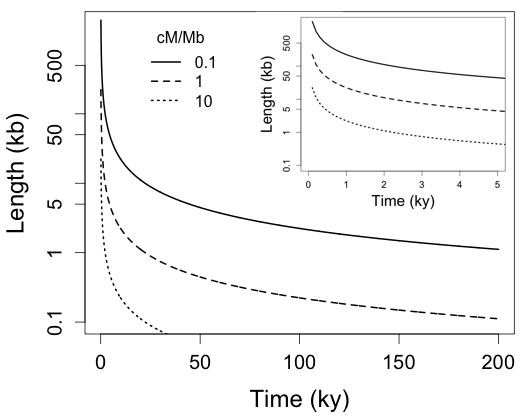
\includegraphics[width=0.5\textwidth]{length_vs_time2}
    \caption{Effect of recombination on the expected length of a shared chromosome segment vs. number of years since divergence or introgression.  Shown are three levels of recombination roughly representing high, average, and low recombination regions of the maize genome.} 
\label{fig:length}
\end{SCfigure}

\subsubsection{Did maize serve as a bridge for gene flow between previously isolated Zea taxa?}
\label{sss:bridge}

Our preliminary analyses identified shared haplotypes in allopatric teosinte taxa, suggesting that maize may have served as a bridge for gene flow between \emph{mexicana} and \emph{luxurians} and potentially other \emph{Zea} taxa (see above).  However, an alternative explanation is that these loci were polymorphic in a common ancestor and continue to segregate due to incomplete lineage sorting.
Simple estimates of the length of shared haplotypes expected to be unbroken by recombination suggest that, over the $\sim 140,000$-generation divergence time between \emph{mexicana} and \emph{luxurians} \citep{Ross-Ibarra2009a}, we might well expect to see shared haplotypes of even several kb in length in low recombination regions of the genome (Figure \ref{fig:length}).
The high-density, genome-wide data generated here will provide an opportunity to test whether observed patterns of haplotype sharing between previously allopatric \emph{Zea} are due to recent introgression from maize.  
If shared haplotypes have come from introgression from maize over the last few thousand years, the genome-wide distribution of shared haplotype lengths should reveal longer shared segments (Figure \ref{fig:length}) than if haplotype sharing is due to incomplete lineage sorting alone.

No high-resolution genetic map currently exists for any teosinte, but the Ross-Ibarra group is currently working on producing such a map for \emph{parviglumis} as part of a different NSF project (\# 1238014), and evidence from comparisons among maize populations finds remarkable stability of the genetic map at a relatively coarse scale \citep{bauer2013} suggesting differences in the genetic map are unlikely to dramatically affect our estimates. 
Will will use our teosinte genetic map or the published NAM map \citep{McMullen2009} to generate an expected distribution of shared haplotype lengths along the genome based on expected divergence times between taxa.

Although the limited sampling in \citet{Ross-Ibarra2009a} only identified shared haplotypes between \zm\ and \zl, maize has been found to hybridize with all species in \emph{Zea} \citep{Wilkes1977}.
We will thus include in our analysis the perennial taxa \emph{Zea diploperennis} (hereafter, \emph{diploperennis}) and \emph{Zea perennis} (herafter \emph{perennis}).  
We will sample 12 individuals from each of two populations of \emph{diploperennis} and \emph{perennis} and genotype these using GBS.
These populations, combined with samples from other teosinte populations included in \ref{sss:adaptive_intro} and \ref{sss:scale}, will provide us with a representative sample of wild teosinte populations from across the Americas.
Shared haplotypes will be identified (see methods in \ref{sss:genomescan}) and compared to the expected distribution of haplotype lengths to look for evidence of recent introgression consistent with the hypothesis that maize has served as a bridge for gene flow among teosinte taxa.
Although we cannot exhaustively test for the presence of such haplotypes in all of maize, we will survey public GBS data of more than $>16,000$  samples (\url{www.panzea.org}) to assess their frequency.

\section*{Broader Impacts}

Our efforts to broaden the impact of the research proposed here will begin within our groups through our commitment to effectively mentor volunteer undergraduate interns as well as graduate students and/or postdoctoral scholars funded by the project. Students and postdocs will receive one-on-one training from the investigators and senior personnel on laboratory, computational, and field research methods.  Mentees will also be encouraged and funded to present their work at scientific conferences.  Our groups have an excellent mentoring track record with four undergraduate students in the last five years publishing their work in scholarly journals and multiple underrepresented minorities participating in our research.

\subsection*{ISU GK12 Fellowship Program}
	
In addition to the student and postdoc mentoring that will occur within our groups, as part of our broader impact activities each year one of our graduate students will participate in Iowa State University's GK12 Fellowship program (\emph{Symbi}; \url{http://www.gk12.iastate.edu/default.asp}; see attached letter of commitment). The selected graduate student will spend one full day each week in a middle or high school science classroom for the entire academic year of the Des Moines Public School District. This is the largest and most diverse school district in Iowa with over 50\% underrepresented minority student enrollment and over 70\% of students receiving free or reduced-cost lunch. The graduate student will introduce the K12 students to the scientific process through inquiry-based activities, relate the students’ science curriculum to real world examples, work with students on their science fair projects, and serve as a role model in a STEM profession. Furthermore, the graduate student will introduce students to his/her research project on hybridization and introgression in \emph{Zea}, a topic that is particularly well suited for teaching evolution in Iowa given the important role that maize plays in the Iowan economy. In introducing his/her dissertation research, the graduate student will engage Des Moines students in how research is conducted and provide STEM content professional training to his/her partner teacher.

The GK12 Fellow will work with approximately 150 students on a regular weekly basis.  Student assessments from the ISU GK12 Fellowship Program have shown that a significant number of students like science more after having a GK Fellow in the classroom.  Teachers report that having a GK12 Fellow in their classroom is excellent professional development.  The PI will also visit the classroom and will support the selected graduate student in their development of appropriate material for the K12 audience.

\subsection*{US-Mexico Exchange Program}
	
Finally, we will establish a student exchange program between the Eguiarte Laboratory at UNAM in Mexico and the Hufford and Ross-Ibarra Laboratories in the United States. The Ross-Ibarra Laboratory has run an NSF-supported, US-Mexico exchange program for the last three years.  All of the exchange students involved in the program have continued on to additional graduate work, and two have earned authorship on forthcoming papers from their internship.  We will build upon the success of this program.  A student from the Eguiarte group will spend 2-3 months in either the Hufford or Ross-Ibarra Laboratory learning the GBS methodology and/or honing his/her skills in population genomic analysis, whereas a student from the Hufford and/or Ross-Ibarra Laboratories will travel to Mexico to participate in sample collection trips and to obtain expertise in common garden field experiments. This exchange will build capacity in all groups involved and will provide a valuable international research experience for a graduate student supported by the grant.  

Senior Personnel Claudia Calderon has previously led international student research trips and will assist in preparing students from both the United States and Mexico for the exchange program. A survey will be given to both exchange students and faculty in order to gauge expectations prior to the trip and facilitate collaborations amongst the labs.  The survey will also assess students' knowledge and preconceived ideas  regarding their travel destinations.  A meeting (online or face-to-face) with the cohort of students traveling will help address these pre-conceptions and reduce cultural misunderstandings.  Suggestions will be given to students of how to prepare before the trip (visa, immigration requirements) and how to communicate with their peers and others during their exchange.  Students will be given information regarding the facilities where they will be staying, transportation to be used, food and water safety, the availability of telecommunications and general safety guidelines.

\required{Results From Prior NSF Support}
% 5 pages or fewer of the 15 pages for entire description document.
% include results from NSF grants received in the past 5 years.
% If supported by more than one grant, choose the most relevant one.

% For each grant, include: 
%	(a) NSF award number, amount, dates of support 
%	(b) The title of this project
%	(c) Publications resulting from this research
%	(d) Summary of the results of the completed work
%	(e) A brief description of data samples available and other research products not described 	      elsewhere
%	(f) For renewed support, a description of the relationship between the completed and 			      proposed work

% Due to space limitations, it is often advisable to use citations rather
% than putting the titles of the publications in the body 
% of this section

\subsection*{Ross-Ibarra: \#1238014: Biology of Rare Alleles in Maize and Its Wild Relatives}
\$13,311,185 (\$2,368,767 to Ross-Ibarra), 05/15/13-04/30/18. PI Edward Buckler, co-PIs J. Doebley, J. Holland, S. Flint-Garcia, Q. Sun, P. Bradbury, S. Mitchell, J. Ross-Ibarra
\par\noindent{\bf Intellectual merit} In the first year we have developed accurate imputation approaches, found evidence for the importance of deleterious variants and non-genic polymorphisms in heterosis and GWAS, documented differences in recombination among the parents of the NAM population, and found population genetic evidence suggesting the importance of demography and purifying selection across the genome.  The grant has produced 18 total publications in its first year (only publications involving PIs Flint-Garcia and Ross-Ibarra are shown below).
\par\noindent{\bf Broader impacts}  In the first year this project has included 10 postdoctoral and 12 graduate trainees. The GBS workshop and traveling maize exhibit continue to be popular and successful. A new version of the teacher-friendly guide to maize evolution has been revised and published online.
\par\noindent{\bf Publications} \citet{peiffer2013genetic, Romay2013, wills2013many, Mezmouk2014, Peiffer2014, sood2014mining}

\subsection*{Ross-Ibarra: \#0922703: Functional Genomics of Maize Centromeres}
\$5,008,031 (\$754,409 to Ross-Ibarra). 09/01/09-08/31/14. PI Kelly Dawe, co-PIs J. Birchler, J. Jiang, G. Presting, J. Birchler, J. Ross-Ibarra\\
\par\noindent{\bf Intellectual merit} Centromeres are regions of the genome that organize and regulate chromosome movement, yet their biology remains poorly understood. Co-PI Ross-Ibarra's group has focused on the evolutionary genetics of centromeres. This work has demonstrated the remarkable evolutionary lability of centromere tandem repeats, but has shown that there is little evidence in maize for coevolution between centromere sequence and kinetochore proteins. Ongoing work seeks to characterize kinetochore proteins, assess the phylogenetic evidence for longer-term coevolution, and understand patterns of centromere and genome size variation in natural populations.\\
\par\noindent{\bf Broader impacts}  Co-PI Ross-Ibarra has established an international student exchange program as part of this grant. Data and result of this project have been disseminated via publications and presentations as well as deposited in the maize genetics community database \url{www.maizegdb.org}. Former trainees on the grant include Dr. Matthew Hufford (PI on the current grant).\\ 
\par\noindent{\bf Publications} \citet{Shi2010a, Chia2012a, Fang2012, Hufford2012, Hufford2012b, Hufford2013, Melters2013a, Kanizay2013, Pyhajarvi2013}

